\documentclass[conference]{IEEEtran}
%\IEEEoverridecommandlockouts
% The preceding line is only needed to identify funding in the first footnote. If that is unneeded, please comment it out.
%Template version as of 6/27/2024

\usepackage{algorithm}
\usepackage{cite}
\usepackage{cprotect}
\usepackage{amsmath,amssymb,amsfonts}
\usepackage{algorithmic}
\usepackage{graphicx}
\usepackage{hyperref}
\usepackage{outlines}
\usepackage{textcomp}
\usepackage{xcolor}
\def\BibTeX{{\rm B\kern-.05em{\sc i\kern-.025em b}\kern-.08em
    T\kern-.1667em\lower.7ex\hbox{E}\kern-.125emX}}
\graphicspath{ {./images/} }

\renewcommand{\algorithmicrequire}{\textbf{Input:}}
\renewcommand{\algorithmicensure}{\textbf{Output:}}
\renewcommand{\algorithmicforall}{\textbf{for each}}
\makeatletter
\newcommand\fs@norules{\def\@fs@cfont{\bfseries}\let\@fs@capt\floatc@ruled
  \def\@fs@pre{}%
  \def\@fs@post{}%
  \def\@fs@mid{\kern3pt}%
  \let\@fs@iftopcapt\iftrue}
\makeatother
\floatstyle{norules}
\restylefloat{algorithm}

\begin{document}

\title{A Lightweight, Swappable Voxel Ray-Tracer}

\makeatletter
\newcommand{\linebreakand}{%
  \end{@IEEEauthorhalign}
  \hfill\mbox{}\par
  \mbox{}\hfill\begin{@IEEEauthorhalign}
}
\makeatother

\author{\IEEEauthorblockN{Ann Gao}
\IEEEauthorblockA{\textit{Dept. Computer Science} \\
\textit{University of Central Florida}\\
Orlando, FL \\
an863834@ucf.edu}
\and
\IEEEauthorblockN{Nathan Hall}
\IEEEauthorblockA{\textit{Dept. Computer Science} \\
\textit{University of Central Florida}\\
Orlando, FL \\
na116376@ucf.edu}
\and
\IEEEauthorblockN{Jonah Henriksson}
\IEEEauthorblockA{\textit{Dept. Computer Science} \\
\textit{University of Central Florida}\\
Orlando, FL \\
jo295297@ucf.edu}
\linebreakand
\IEEEauthorblockN{Christopher Jenkins}
\IEEEauthorblockA{\textit{Dept. Computer Science} \\
\textit{University of Central Florida}\\
Orlando, FL \\
ch119158@ucf.edu}
\and
\IEEEauthorblockN{Felipe Schmidt}
\IEEEauthorblockA{\textit{Dept. Computer Science} \\
\textit{University of Central Florida}\\
Orlando, FL \\
fe805154@ucf.edu}
}

\maketitle

\begin{abstract}
Voxel rendering is a technique for visualizing 3D volumes, with applications in medical technology, terrain visualization, and video games.
Simple voxel rendering implementations rely on “meshing”, a process by which the volume is converted to a mesh for rasterization.
For many tasks, this is sufficient, but also suffers from memory constraints which prevents meshing from scaling to large scenes (since both the voxel data and heavy mesh representation has to be stored).
An alternative solution that lacks such constraints is ray-tracing; which operates on the voxel data itself.
In this project, we present a CPU voxel ray-tracer implemented in Rust, alongside two storage solutions that can be swapped: a dense array-backed storage, and a sparse octree storage.
The relative performance of these solutions are assessed via render benchmarks.
\end{abstract}

\begin{IEEEkeywords}
voxels, ray-tracing, octree.
\end{IEEEkeywords}

\section{Introduction}
The term “voxels” is derived from the term “pixels”: where a “pixel” is a “\textbf{pic}ture \textbf{el}ement” that represents part of a picture, a “voxel” is a “\textbf{vo}lume \textbf{el}ement” that represents part of a volume.
Volumetric data can range from MRI slices to point clouds to generated volumes in video games.
Voxels are a representation of this volumetric data in a grid structure, just as pixels store raster images in a grid structure.
However, while pixels and voxels are similar in structure, the way they are visualized differs vastly.
Pixels can simply be drawn to a screen surface, but voxels are points in 3D space and drawing techniques can either draw the individual points, as with point cloud rendering, or the isosurface, which is the concern of this paper.

Isosurface rendering is the ubiquitous form of voxel rendering, to the point that “voxel rendering” almost always refers to rendering the isosurface of a voxel grid.
The isosurface of a voxel grid is the surface present between voxels that surpass some threshold and those which don’t (i.e. the boundary between voxels that are “present” and those which aren’t).
To render such an isosurface, the approach varies on the underlying render technique used.
Such render techniques generally fall into two categories: rasterization and ray-tracing.

Ray-tracing is the earliest method of rendering, which works by simulating rays of light in a scene, making it capable of rendering realistic images.
However, it is computationally expensive, leading to the popularity of another method for real time applications: rasterization.
Rasterization works by projecting triangles of a polygonal mesh onto the camera’s 2D view and filling in their bounds using small programs called “shaders”.
Because of the strengths and weaknesses of both methods, voxel rendering techniques fall into two categories as well: isosurface mesh extraction for rasterization and voxel traversal for ray-tracing (there are also hybrid techniques, but they exist as an optimization of voxel traversal).

Isosurface mesh extraction, popularly known as “meshing”, is the process of converting voxels to a mesh of the isosurface, and there are many meshing algorithms, such as “greedy meshing”, “marching cubes”, “naive surface nets”, etc.
All have their own characteristics making them suitable for particular applications.
However, when rendering large scenes, meshing and rasterization typically struggle to scale in performance.
Meanwhile, ray tracing is capable of scaling in performance, due to optimizations that are relatively easy to implement with ray tracing, such as acceleration structures and LOD (level-of-detail), and the lack of a mesh generation step when updating voxels, as well as better memory scaling (storing a mesh takes up memory on top of storing the voxel volume).
Because of this difference in scaling potential, when rendering large scenes on mid to high end consumer computers, ray tracing becomes more performant than rasterization.

\begin{figure}[htbp]
\centerline{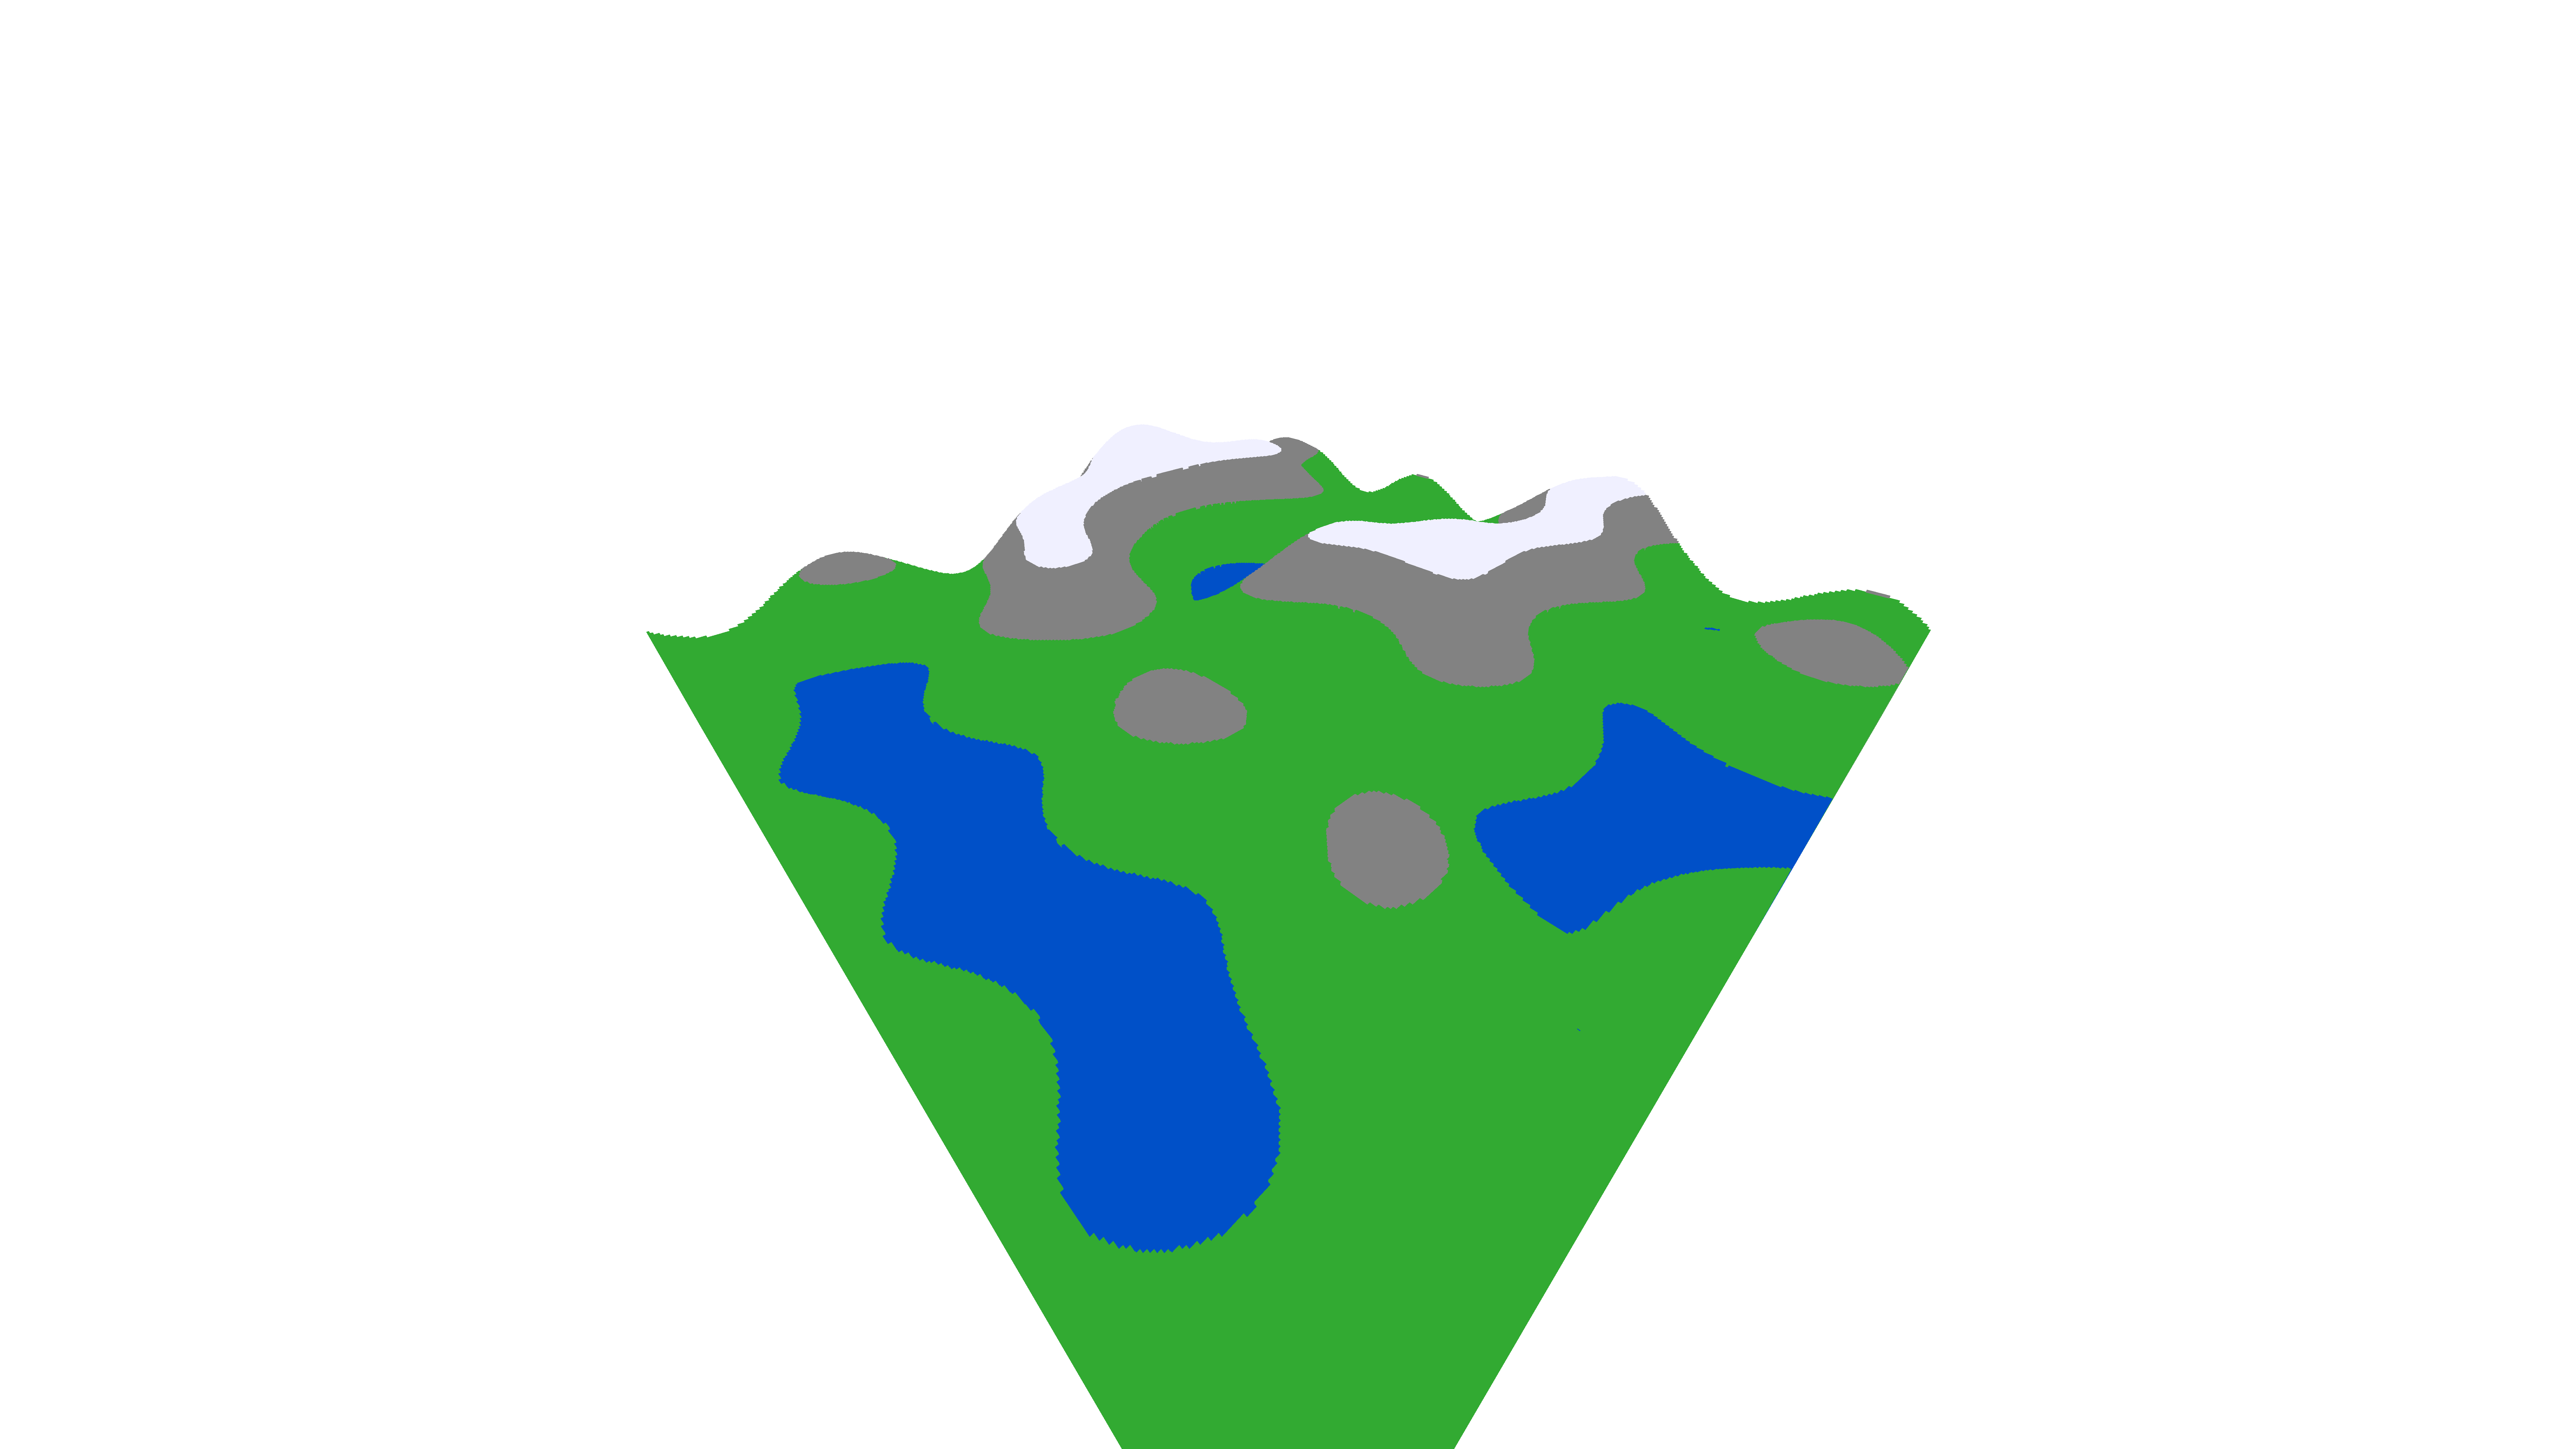
\includegraphics[width=\linewidth]{render}}
\caption{A render produced by our voxel ray-tracer.}
\label{render}
\end{figure}

\subsection{Problem Statement}

\textbf{We have achieved the goal for this project: implement a CPU voxel ray-tracer in the Rust language with two storage backends: a dense array storage and a sparse voxel octree storage, and benchmark them against each other.}
The dense array represents a naive voxel storage implementation, while the sparse octree represents an acceleration structure implementation: an optimization for ray traversal via a space partitioning structure.
Using both storage solutions, we can assess the benefits of octrees for optimizing ray traversal in voxel scenes via benchmarks simulating rendering scenes at different sizes and resolutions.
See Fig.~\ref{render} for an example render produced by our voxel ray-tracer.

\section{Methodology}

By making the ray tracer generic over storage backends, we can swap between ray tracing implementations.
To assess the performance of each implementation, the benchmarks will consist of measuring the time it takes for each implementation to render a scene for a given scene size and frame resolution.

\section{Implementation}

The program is divided into the following parts:

\begin{outline}
\1 Voxel Generator
\1 Scene Object with Swappable Storage Backends
\2 Dense Array-Backed Storage
\2 Sparse Octree-Backed Storage
\1 Framebuffer
\1 Camera Controller
\1 Ray Tracer
\1 Image Exporter
\1 Command Line Interface
\end{outline}

The clear boundaries between components was beneficial to dividing work among colleagues.

\subsection{Voxel Generation}

[Elaborate on voxel generation]

\subsection{Scene Object}

The scene object stores the scene and provides an interface for ray tracing.
Our project has two scene object implementations: a dense array-backed storage object and a sparse octree-backed storage object.
There is some overlap in the implementations of these objects, particularly the \verb|Scene| trait, \verb|Ray| struct, and \verb|IAabb| struct:

\cprotect\subsubsection{\verb|Scene| trait}

The \verb|Scene| trait has two items: a function for creating the scene object given the voxel generator and a method for tracing a ray through the scene.
This is the interface from which the ray tracer interacts with the scene.

\cprotect\subsubsection{\verb|Ray| struct}

The \verb|Ray| struct is a vector pair of the ray origin and the ray direction.
It is used to simulate light rays that traverse the scene from the camera.

\cprotect\subsubsection{\verb|IAabb| struct}

The \verb|IAabb| struct represented an axis-aligned bounding box (AABB) represented by integer vectors.
By iterating over every coordinate in an AABB, the storage backend can query the voxel generator for a voxel and store it if present.

An AABB can also be used during a ray trace, as a quick intersection test for the entire volume.
The algorithm used for fast intersection tests is from "An Efficient and Robust Ray-Box Intersection Algorithm" by Williams et al. \cite{williams}
To summarize how the algorithm works: it takes advantage of properties observed in intersection between rays and AABBs to quickly check if the ray crosses the box boundaries.

A more detailed but brief explanation is that the algorithm projects boundary line intersections to a 1D line representing distance traveled across the ray and checks the order of these intersections to verify that the ray enters all bounds before exiting any other bounds (See Fig.~\ref{fast-intersection} for an example of the calculations).

\begin{figure}[htbp]
\centerline{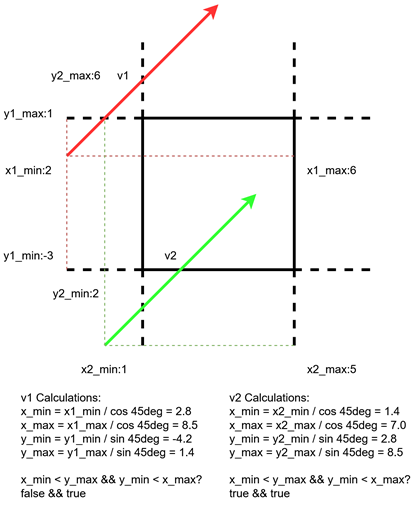
\includegraphics[width=\linewidth]{fast-intersection}}
\caption{Two example calculations for fast ray-box intersections using 2D coordinates.}
\label{fast-intersection}
\end{figure}

\subsection{Dense Storage}

The dense storage backend stores every possible position in the voxel volume in a single array.
It is most beneficial to use such a storage solution when most positions hold present voxels, or in other words, is densely populated, hence the name.

\begin{figure}[htbp]
\centerline{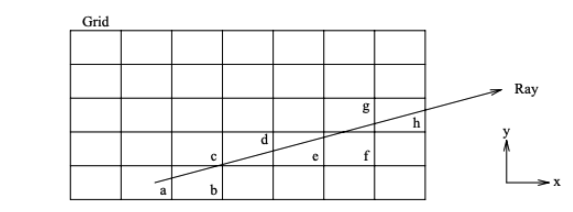
\includegraphics[width=\linewidth]{fast-traversal}}
\caption{The fast voxel traversal algorithm in action.}
\label{fast-traversal}
\end{figure}

For the dense storage backend, there exist many algorithms for ray tracing through a multidimensional array, but most are based on the “Fast Voxel Traversal” algorithm by Amanatides and Woo, which will be what we use for ray tracing in the dense storage backend \cite{amanatides}.
This algorithm works by tracking the index and position for each axis and moving the ray along the axis with the shortest distance to the next index (See Fig.~\ref{fast-traversal}).
By doing so, it ensures that no voxels are missed during iteration while not testing positions that don't intersect the ray.
When a voxel is found or the indices go out of bounds, it returns.

\subsection{Sparse Storage}

The sparse storage backend stores present voxels in a space partitioning structure called an "octree" (See Fig.~\ref{octree} for examples).
It is most beneficial to use such a storage solution when there are large gaps in the volume, or in other words, when the volume is sparsely populated, hence the name.

\begin{figure}[htbp]
\centerline{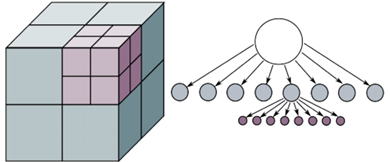
\includegraphics[width=\linewidth]{octree}}
\caption{Two example visualizations of an octree.}
\label{octree}
\end{figure}

Octrees are tree structures that have branches that subdivide space along each axis, allowing for traversing over "octants", the 8 subdivisions of each branch.
The benefit is that octants that don't contain voxels are culled, meaning that entire areas of empty space can be skipped when a ray traverses the octree.

An easy way to understand ray traversal through octrees is to examine ray traversal for their 2D counterpart: quadtrees, which subdivides 2D space into quadrants (See Fig.~\ref{quadtree}).

When beginning ray traversal, the first quadrant to check is the one where the ray originates in the direction of (so compare the volume origin to the ray origin).
If the quadrant has children, the algorithm is recursively called for that quadrant.
Otherwise, other quadrants are checked if the ray crosses the respective local origin's axes (the local origin is the origin of the volume for the top level and origin of quadrants for recursive calls) and in order of the distance required to cross the local origin.

\begin{figure}[htbp]
\centerline{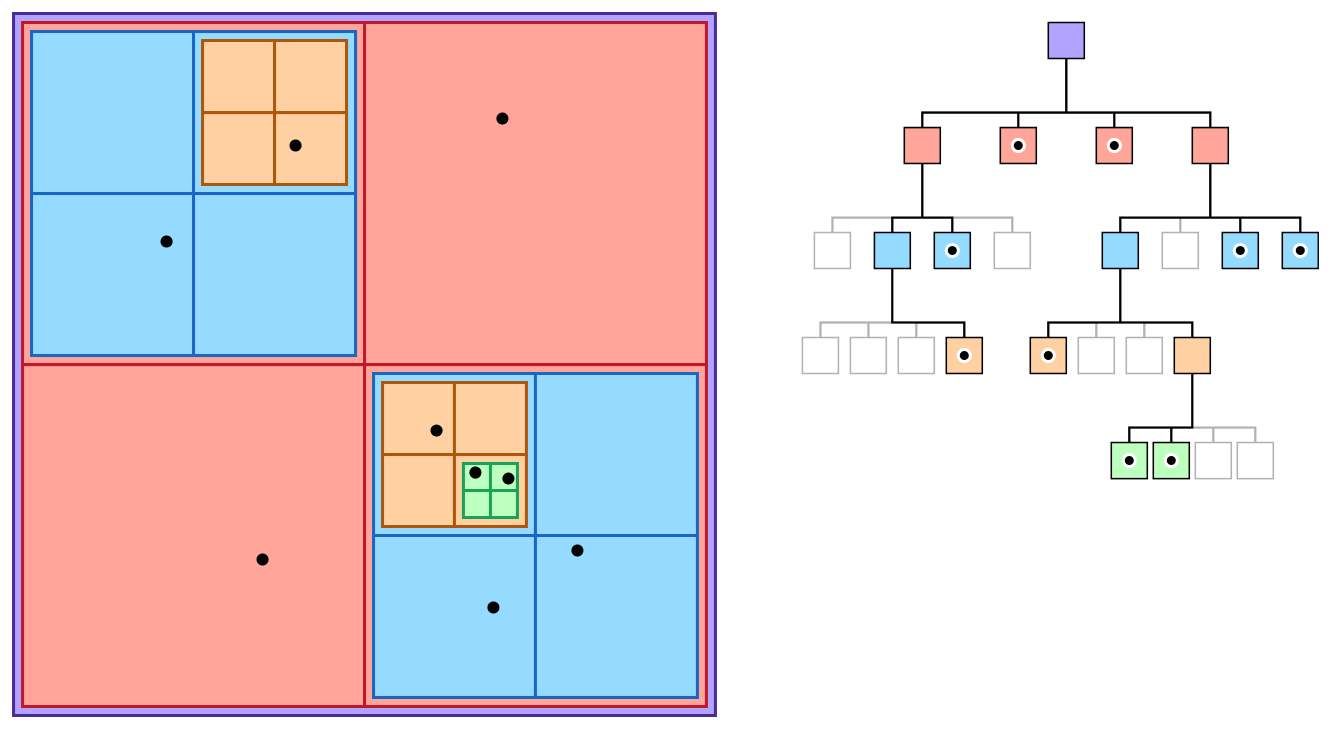
\includegraphics[width=\linewidth]{quadtree}}
\caption{Two example visualizations of a quadtree (note: this example shows variable depth for storing items, while our octree implementation has a constant depth).}
\label{quadtree}
\end{figure}

In order to visualize octree traversal, a debug mode was added to the ray tracer, which renders the edges of bounding boxes and colors voxels black (See Fig.~\ref{debug}).

\begin{figure}[htbp]
\centerline{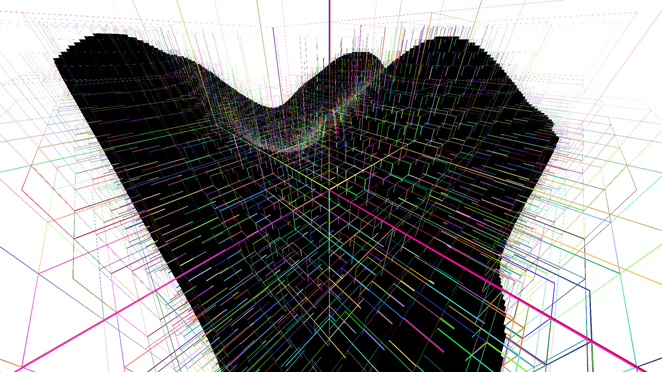
\includegraphics[width=\linewidth]{debug}}
\caption{An octree structure visualization for debugging.}
\label{debug}
\end{figure}

It renders the edges by running face intersection tests for the ray and checking if any of the intersection points are within some threshold (that is, if two points on separate faces are close to each other, then they must lie near the edge that joins both faces).
The color for the edge is picked via Pearson hashing, a simple hashing algorithm for small inputs that also produces byte-sized hashs via a lookup table (See Alg.~\ref{pearson} for the generic algorithm).
The algorithm was modified to consume bytes from a position vector and produce three bytes corresponding to color channels.

\subsection{Framebuffer and Image Exporter}

Once we have processed all the scene information, it is time to save it to an image so we can view it.
We do this by adding information to a framebuffer, then copying the framebuffer into a PNG file.
The framebuffer is a data structure that holds all the image information of the rendered scene.
It contains a memory reference to a heap-allocated array of 4-byte integers for each pixel.
Each integer represents the RGBA values of a pixel, with the first byte holding the R value, second byte holding the G value, etc.
The array uses an atomic data type, which allows for multiple threads to access and modify the values of different pixels safely and concurrently to allow faster image generation.
We use Rust’s \verb|image| crate to then write to an image file specified by a given output path.

\subsection{Camera Controller}

[Elaborate on camera and ray instantiation]

\subsection{Ray Tracer}

The ray tracer brings together the scene object, camera, and framebuffer components to provide an render method that generates a new framebuffer with contents rendered from the scene object with rays instantiated by the camera.
The ray tracer runs in parallel with help from the \verb|rayon| crate, which provides traits for parallel iterators.
\verb|rayon|'s parallel iterators work by splitting an iterator across threads via work-stealing, so if a thread finishes it's work before another, it can split the iterator on another thread to keep itself busy.

What the ray tracer needs to iterate over is the pixel coordinates and values, in order to instantiate rays using the coordinates and save the result to the value.
To do this, we implemented a parallel iterator for the framebuffer that produces \verb|PixelRef| objects, that store the coordinates and references to the pixel value.

This requires implementing three components: \verb|ParIter| (our parallel iterator), \verb|ParIterProducer| (our iterator producer, which is able to split itself and convert into an iterator), and \verb|Iter| (our normal iterator which individual threads run).
The flow of information can be roughly modeled as $\verb|Framebuffer| \to \verb|ParIter| \to \verb|ParIterProducer| \to \verb|Iter| \to \verb|PixelRef|$.

For each \verb|PixelRef| we run a task which instantiates a ray from the camera using the pixel coordinates, calls the \verb|trace| method on the scene object with that ray, and saves the result to the value reference, after first converting the color vector to an unsigned integer.

\subsection{Command Line Interface}

[Elaborate on the CLI]

\section{Evaluation}

To evaluate the performance benefits of sparse voxel octrees over array-backed storage, we constructed benchmarks via \verb|criterion.rs| that measured the performance of each storage backend over scene size and frame resolution.
The benchmarks ran across 12 threads on a mid-range consumer PC with an AMD Ryzen 5 2600 6-core CPU and 32GB of RAM.

\begin{table}[htbp]
\caption{1080p Resolution Benchmarks}
\begin{center}
\begin{tabular}{|c|c|c|c|}
\hline
\textbf{Scene Size} & \textbf{Dense} & \textbf{Sparse}  & \textbf{Ratio} \\\hline 
50 & 37.557 ms & 211.86 ms & 0.1773 \\\hline
100 & 192.48 ms & 247.86 ms & 0.7766 \\\hline
250 & 811.93 ms & 122.55 ms & 6.6253 \\\hline
\end{tabular}
\label{1080p-bench}
\end{center}
\end{table}

\begin{table}[htbp]
\caption{4k Resolution Benchmarks}
\begin{center}
\begin{tabular}{|c|c|c|c|}
\hline
\textbf{Scene Size} & \textbf{Dense} & \textbf{Sparse}  & \textbf{Ratio} \\\hline 
50 & 261.11 ms & 2.5230 s & 0.1035 \\\hline
100 & 3.0203 s & 3.5526 s & 0.8502 \\\hline
250 & 10.016 s & 2.0995 s & 4.7706 \\\hline
\end{tabular}
\label{4k-bench}
\end{center}
\end{table}

The benchmarks assessed the storage backends for small and medium scenes, with sizes of 50, 100, and 250 voxel extents (the total volume is $(2x)^3$ voxels for each $x$ size), and for resolution of 1080p ($1920 \times 1080$ pixels) and 4k ($7680 \times 4320$ pixels).
We only tested small and medium sized scenes since the time to render larger scenes took too long to collect samples for in a practical time for iterating modifications.
The camera for each scene was located in the top corner of the scene, facing inwards toward the origin (from a position of $(x-10)\hat{v}$).
The results are the average time to render a scene, for 100 samples.

For small scenes, the dense storage solution was faster, but that quickly changed as scenes grew in size.
For scenes with size 250, the sparse storage solution was incredibly fast, even faster than it was for smaller scenes.
This was due to the voxel generation having a height limit of 100, which meant for larger scenes that there was more empty space.
Since the sparse backend benefits from empty space, it was able to skip more empty space, leading to faster render times.

See Fig.~\ref{violin} for violin plots.

\begin{figure}[htbp]
\centerline{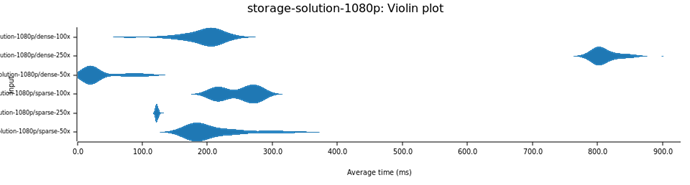
\includegraphics[width=\linewidth]{violin-1080p}}
\centerline{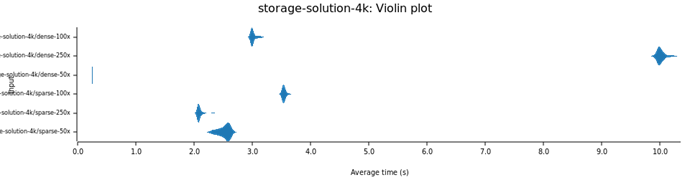
\includegraphics[width=\linewidth]{violin-4k}}
\caption{Violin plots of the benchmarks.}
\label{violin}
\end{figure}

\subsection{Tracing}

To allow for further optimization, tracing instrumentation was added to the program with the \verb|tracing|, \verb|tracing-subscriber|, and \verb|tracing-tracy| crates, which allow for timing functions using the \href{https://github.com/wolfpld/tracy}{Tracy profiler}.
From that, we can see where the program spends the most time in and look for ways of shaving time off in those areas (See Fig.~\ref{tracing} for an example).

\begin{figure}[htbp]
\centerline{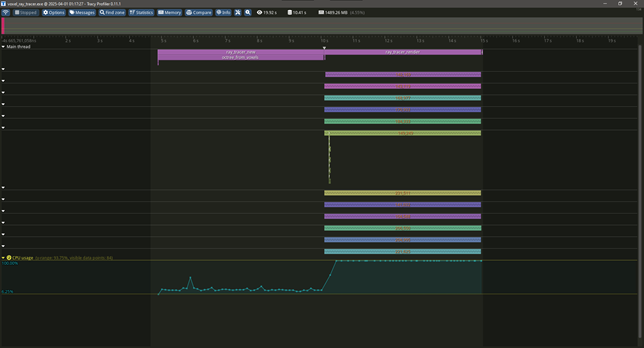
\includegraphics[width=\linewidth]{tracing}}
\caption{An example of collected traces (notice that half the time of the program is spent constructing the scene on a single thread).}
\label{tracing}
\end{figure}

Generating traces is costly, so this feature was put behind a feature flag.

\section{Conclusion}

[Draw some conclusion that affirms that we did what we set out to do]

\begin{thebibliography}{00}
\bibitem{williams} Williams, Amy \& Barrus, Steve \& Morley, R. \& Shirley, Peter. (2005). An Efficient and Robust Ray-Box Intersection Algorithm. J. Graphics Tools. 10. 49-54. 10.1145/1198555.1198748. 
\bibitem{amanatides} Amanatides, John \& Woo, Andrew. (1987). A Fast Voxel Traversal Algorithm for Ray Tracing. Proceedings of EuroGraphics. 87.
\end{thebibliography}

\begin{algorithm}[H]
\caption{Generic Pearson Hashing Algorithm}
\begin{algorithmic}[1]
\REQUIRE Byte array $C$
\ENSURE Byte-sized hash $h$
\\ \textit{Initialisation} : $T$ is a permutation of an array containing bytes 0 to 255
\STATE $h \gets 0$
\FORALL{$c \in C$}
\STATE $h \gets T[h \oplus c]$
\ENDFOR
\RETURN $h$
\end{algorithmic}
\label{pearson}
\end{algorithm}

\end{document}
